\chapter{Validierung}
\label{Validierung}

Ein Ziel der Diplomarbeit ist die Entwicklung einer nutzerfreundlichen Oberfläche zur Problemlösung in modularen Anlangen. Dieses Kapitel bewertet die Qualität der Umsetzung. Dazu werden zunächst die definierten Anforderungen an das Assistenzsystem ausgewertet. Die Anforderungen beschreiben nur die Funktionalitäten und geben keinen Hinweise auf eine gute Gestaltung des Assistenzsystems. Für die Bewertung der Gestaltung wird der Prototyp unter anderem mit den Grundsätzen der Dialoggestaltung und den Aspekten für die Informationsdarstellung verglichen. Mit einer Umfrage unter Experten kann abschließend eingeschätzt werden, wie nutzerfreundlich das System ist, welche Funktionen noch verbessert werden müssen \todo{was noch?}  und ob es Anwendung findet.

\section{Vergleich mit Anforderungen}
In Abschnitt \ref{3:Anforderungen} wurden Anforderungen an das Assistenzsystem gestellt. Die Erfüllung der Anforderungen wird im Folgenden diskutiert. Eine erste Einschätzung gibt jeweils eine Tabelle. Ein \textbf{+} bedeutet voll erfüllt, ein \textbf{o} bedeutet teilweise erfüllt und ein \textbf{-} bedeutet nicht erfüllt.

\subsection{Unterstützung der Problemidentifikation}
Der Nutzer soll bei der Problemidentifikation unterstützt werden. Tabelle \ref{tab:Anforderungen-Problemidentifikation} stellt dar, wie gut die einzelnen Anforderungen durch den Prototypen erfüllt sind.
\begin{table}[htbp]
\caption{Auswertung Anforderungen Problemidentifikation}
\centering
\begin{tabular}{l|c|c|c|c|c|c}
\textbf{Anforderung} & PI 1.1 & PI 1.2 & PI 1.3 & PI 2 & PI 3 & PI 4 \\
\hline
\textbf{Erfüllt} & o & + & o & + & + & + \\
\end{tabular}
\label{tab:Anforderungen-Problemidentifikation}
\end{table}

Insgesamt ist die Unterstützung der Problemidentifikation als positiv zu werten. Es gibt lediglich noch Anpassungsbedarf bei der Problembeschreibung. Dem Nutzer wird aktuell nicht die Möglichkeit gegeben, selber ein Problem zu melden. Weitere Details und Begründungen zu der Bewertung sind im Folgenden erläutert.

\subsubsection*{PI 1.1 Problembeschreibung}
Dem Nutzer sollte die Möglichkeit gegeben werden, das Problem zu beschreiben. Der Prototyp erfüllt dieses, indem sowohl textuell die Beschreibung verändert werden kann, als auch die Parameter der Rahmenbedingung verändert werden können. Ein Beispiel dafür ist die Wartungsdauer. Der Nutzer kann in Absprache mit dem Hersteller festlegen, wie lange die Wartung für das Modul dauert.

Hat der Nutzer selber ein Problem entdeckt, ist es derzeit nicht möglich dieses zu beschreiben. Dafür muss zunächst näher untersucht werden, welche Probleme die modulare Anlage nicht selber erkennt und durch den Nutzer gemeldet werden müssen. Das könnten beispielsweise Flüssigkeiten sein, die auslaufen oder ungewöhnliche Geräusche, die nicht durch Sensoren erfasst werden können. Erste Ideen gab es dazu bereits in \cite{Bieber2018}. Es ist zu prüfen, ob diese Ansätze auch für die modularen Anlagen umgesetzt werden können.

\subsubsection*{PI 1.2 Zieldefinition}
Dem Nutzer sollte die Möglichkeit gegeben sein, die Ziele zu definieren, um anhand dieser die Lösungen zu finden. Der Prototyp erfüllt diese, indem sich die Parameter der Ziele verändern und neue Ziele hinzufügen lassen.

\subsubsection*{PI 1.3 Informationen}
In den Anforderungen steht, dass dem Nutzer alle relevanten Informationen über die aktuelle Situation zur Verfügung stehen sollen. Die Auswertung dieser Anforderung gestaltet sich sehr schwierig, da die Anforderung sehr unspezifisch formuliert ist.

Abgeleitet aus der Analyse ist mit allen relevanten Informationen Folgendes gemeint:
\begin{itemize}
\item Aktueller Zustand der Anlage: Verschaltung der Module, KPIs, Rezept, Services
\item Informationen über den Produktionsprozess, z. B.:
	\begin{itemize}
	\item Wie sehr ist die aktuelle Anlage ausgelastet?
	\item Wie gut ist die Qualität meiner Produktion?
\end{itemize}
\end{itemize}

Der aktuelle Zustand der Anlage wird durch die PFE und damit auch durch Prototypen angezeigt. Die Informationen über den Produktionsprozess können über die Key Perfomance Indicator abgedeckt werden. Es ist bis jetzt allerdings nicht eindeutig, wo und wie diese definiert werden. Daher ist auch nicht eindeutig, ob damit die Anforderung vollständig erfüllt ist. Für eine detaillierte Bewertung muss genau festgelegt sein, welche KPIs angezeigt werden sollen und welche Informationen über den Produktionsprozess relevant sind. Beides ist stark von den Bedürfnissen des Betreibers der modularen Anlage abhängig. Aus diesem Grund ist die Anforderung allgemein als erfüllt zu bewerten, da die grundlegenden Informationen abgedeckt werden.

%Der aktuelle Prototyp stellt den aktuellen Zustand modularen Anlage dar und erfüllt damit den ersten Teil der Anforderung. Ein Produktionsprozess kann noch durch weitere Faktoren beeinflusst werden. Relevant sind auch die Umgebungsbedingungen, wie die Umgebungstemperatur, und die Mitarbeiter, die an der Anlage arbeiten. Diese Informationen können als weitere Daten in die Problembeschreibung mit einfließen. 

\subsubsection*{PI 2 Unterstützung bei Problemidentifikation}
Das Assistenzsystem unterstützt den Nutzer bei der Problemidentifikation mit Meldungen, Warnungen und Alarme. Dadurch wird der Nutzer auf Probleme aufmerksam gemacht.

\subsubsection*{PI 3 Ziele hinzufügen}
Der Nutzer hat im Feld der Problembeschreibung die Möglichkeit für ihn relevante Ziele hinzuzufügen und irrelevante Ziele zu löschen.

\subsubsection*{PI 4 Problembereich}
Dem Nutzer wird der Auslöser des Problems durch die Problembeschreibung mitgeteilt. Der Problembereich wird hervorgehoben, indem irrelevante Informationen durch graue halbdurchsichtige Felder verdeckt werden.

\subsection{Unterstützung bei der Problemlösung}
Die Anforderungen für die Unterstützung bei der Problemlösung sind nur teilweise erfüllt. Hintergrund ist einerseits die fehlende Möglichkeit im Prototyp eigene Lösungen hinzuzufügen. Es muss dafür noch untersucht werden, welche Eingaben der Nutzer tätigen möchte. Andererseits sieht der Nutzer nicht, wie sich seine Entscheidung auf die Produktqualität auswirkt. Eine Übersicht auf die Auswirkungen der Produktionsziele und der Struktur der Anlage wird durch die Assistenz bereitgestellt. Diese unterstützt den Nutzer durch eine Vorauswahl an Lösungen.

\begin{table}[htb]
\caption{Auswertung Anforderungen Problemlösung}
\centering
\begin{tabular}{l|c|c|c|c|c}
\textbf{Anforderung} & PL 1 & PL 2 & PL 3.1 & PL 3.2 & PL 4 \\
\hline
\textbf{Erfüllt} & + & o & o & o & - \\
\end{tabular}
\label{tab:Anforderungen-Problemlösung}
\end{table}

\subsubsection*{PL 1 Assistenz schlägt Lösungen vor}
Das Assistenzsystem wertet die definierten Ziele des Nutzer aus und sucht aus einem Pool an möglichen Lösungen die Besten aus. Dazu kann auch eine virtuelle modulare Anlage hinzugezogen werden, um vorab mögliche Fehlentscheidungen zu filtern. Die identifizierten Lösungsmöglichkeiten werden dem Nutzer zur Verfügung gestellt. Im Falle des Prototypen sind die Lösungen vordefiniert. Für zukünftige Arbeiten ist es interessant zu erfahren, welche Möglichkeiten zur Lösungsfindung im Rahmen der modularen Anlage existieren. Dabei ist der Unterschied zwischen modulspezifischen und anlagenspezifischen Problemen zu betrachten. Modulspezifisch bedeutet, dass sich das Problem auf das konkrete Modul bezieht und es irrelevant ist, mit welchen anderen Modulen eine Verbindung besteht. Anlagenspezifische Probleme sind nur im Kontext aller verbundenen Module zu beurteilen. Wenn die Module also anders verbunden werden, ändern sich auch die Zusammenhänge von Problem und Lösungen.

\subsubsection*{PL 2 Nutzer schlägt Lösungen vor}
Dem Nutzer soll es möglich sein, selber Lösungen vorzuschlagen. Durch das Plus-Symbol im Reiter Lösungen ist das angedacht, aber nicht ausgeführt. Um sich Gedanken zu machen, wie Lösungen eingegeben werden können, muss im ersten Schritt geklärt werden, was der Nutzer eingeben möchte. Im Rahmen des Modultauschs sollte es möglich sein, noch andere Module in Erwägung zu ziehen. Es ist zu prüfen, ob der PEA-Manager von Jan Funke \cite{Funke2018} eingebunden werden kann. Dadurch hat der Nutzer die Möglichkeit selber nach Modulen zu suchen. Die Tatsache, dass ein Mensch auch kreative Lösungen entwickeln kann, bietet eine ungeahnte Menge an Möglichkeiten und führt zu neuen Herausforderungen. Es ist nicht vorhersehbar, welche Ideen der Nutzer entwickelt. Mit Sicht auf den Use Case hat der Nutzer beispielsweise die Idee, eine andere Anlage vorübergehend still zu legen und ein Modul aus dieser zu nutzen. Solche und weitere Ideen machen das Design von Eingabemöglichkeiten sehr komplex und sind getrennt von dem entwickelten Prototypen zu betrachten.

\subsubsection*{PL 3.1 Auswirkung auf Anlage / Prozess}
Der Prototyp zeigt dem Nutzer an, welche Veränderungen sich in der modularen Anlage durch die Lösung ergeben. Es werden Veränderungen im Rezept, in der Navigation und in den Services angezeigt. Die verfahrenstechnischen Auswirkungen auf den Prozess sind nicht dargestellt. Es ist also nicht abschätzbar, wie sich die Produktqualität durch die Lösung verändern könnte. Die Anbindung an eine virtuelle modulare Anlage, die mögliche Veränderungen berechnet und dem Nutzer mitteilt, ist noch zu entwickeln.

\subsubsection*{PL 3.2 Einflussfaktoren}
Dem Nutzer wird durch das Assistenzsystem angezeigt, welche Einflussfaktoren sich zahlenmäßig unterscheiden. Im Konzept ist vorgesehen, dass alle relevanten Einflussfaktoren sichtbar sind (vgl. \ref{3:Anforderungen}). Relevant bedeutet, dass die Einflussfaktoren zuvor von dem Unternehmen oder dem Mitarbeiter als wichtig definiert wurden.

Die notwendige Darstellung von Serviceabhängigkeiten ist in xx \todo{Verweis} thematisiert, jedoch nicht umgesetzt. Für einen sinnvollen Entwurf ist noch zu untersuchen, wie stark Services voneinander abhängen können. Darauf aufbauend kann dann eine gute Darstellung entwickelt werden. Der Fokus dieser Arbeit richtet sich auf die Modulebene. Auf dieser werden die Einflüsse auf das Rezept und die Services durch Hervorhebung dargestellt.

\subsubsection*{PL 4 Lösungen bewerten}
In den Anforderungen ist definiert, dass der Nutzer die einzelnen Lösungen bewerten kann, um eine Entscheidung zu treffen. Diese Anforderung wurde nicht umgesetzt, da eine Lösung nicht richtig oder falsch sein kann. Es ist möglich, dass eine Lösung besser oder schlechter ist. Die Bewertung dieser ist von der Gesamtsituation (z. B. verfügbare Mitarbeiter, Auftragslage) und dem Wissen des Mitarbeiters abhängig. Diese Anforderung ist daher kritisch zu hinterfragen. Bei Rückblick auf den allgemeinen Problemlöseprozess ist sichtbar, dass Lösungen erst nach Durchführung bewertet werden. Erst dann ist eindeutig, welchen Einfluss die Entscheidung hat. Aus diesem Grund ist eine Bewertung erst nach Anwendung der Lösung sinnvoll.

\subsection{Klustern von Problemen}
Probleme sollen geklustert werden, damit mehrere Probleme parallel bearbeitet werden können. Wie Tabelle \ref{tab:Anforderungen-Probleme} zeigt, sind die Anforderungen erfüllt. Das Assistenzsystem sortiert die Probleme automatisch und macht damit den Nutzer auf das wichtigste aufmerksam.

\begin{table}[htbp]
\caption{Auswertung Anforderungen: Probleme klustern}
\centering
\begin{tabular}{l|c|c|c}
\textbf{Anforderung} & KP 1 & KP 2 & KP 3\\
\hline
\textbf{Erfüllt} & + & + & + \\
\end{tabular}
\label{tab:Anforderungen-Probleme}
\end{table}

\subsubsection*{KP 1 Mehrere Probleme bearbeiten}
Damit ein Problem weiter bearbeitet werden kann, wenn ein neues Problem in den Vordergrund rückt, wurde eine entsprechende Anforderung definiert. Laut dieser sollen mehrere Probleme parallel bearbeitet werden können. Das ist auch relevant, wenn eine Entscheidung für ein Problem nicht sofort getroffen werden muss. Der Nutzer kann das Problem später weiter bearbeiten und sich in der Zwischenzeit einem anderen zuwenden. Die Interaktionsplattform macht das durch die linke Seitenleiste möglich, in der das zu bearbeitende Problem ausgewählt werden kann. 

\subsubsection*{KP 2 Probleme sortieren}
Da im Prototyp nur ein Problem realisiert ist, erfolgt keine konkrete Sortierung der Probleme. Das Konzept sieht jedoch eine Sortierung anhand von Zeit, Komplexität und Arbeitsaufwand vor, wodurch die Anforderung erfüllt ist. Darauf aufbauend kann untersucht werden, ob diese Sortierung im Umgang mit vielen Problemen ausreichend ist.

\subsubsection*{KP 3 Merkmale der Probleme}
Derzeit versieht das Assistenzsystem die Probleme mit den Merkmalen gemäß der definierten Anforderungen. Die Merkmale orientieren sich an der Definition von komplexen Problemen und den Einflussfaktoren in einem Unternehmen. Ob diese für den Nutzer ausreichend sind, ist noch zu prüfen.

\section{Aspekte des Assistenzsystems}
Neben den individuell definierten Anforderungen an die Funktionen des Assistenzsystems, gibt es eine Reihe an Faktoren, die in der Literatur beschrieben sind. Im Folgenden ist eingeordnet, welchen Automatisierungsgrad das Assistenzsystem hat und welche Aufgaben von technischer Assistenz unterstützt werden. Auch die Anforderungen an ergonomisch gute Gestaltung und die Notwendigkeit von Individualisierung werden ausgewertet.

\subsection*{Eingliederung in Automatisierungsgrad}
Abschnitt \ref{3:Anpassung-Aufgabe} macht deutlich, dass sich das Assistenzsystem anhand des Zeitdrucks anpassen soll. Im Prototypen ist das Problem nicht zeitkritisch und sieht daher einen geringen Automatisierungsgrad vor. In die 10 Level der Automatisierung von Sherdian \cite{Wandke2005} lässt sich der Prototyp auf Level 3 einordnen. Bei einem höheren Zeitruck sind auch die Stufen 4 und 5 in Betracht zu ziehen. Level 6 ist im Sinne der kollaborativen Assistenz nicht anzuwenden, da auf diesem Level die Möglichkeiten des Nutzers stark eingeschränkt sind. Es ist noch zu untersuchen, in welchen Problemfällen welcher Autonomiegrad angewendet wird. Dazu sollten auch die Autonomiestufen in der Prozessindustrie von Schegner \cite{Schegner2017} betrachtet werden. In dieses System lässt sich der Prototyp auf Stufe 1 einordnen.

\subsection*{Aufgaben von digitaler Assistenz}
Digitale Assistenz kann eine ganze Reihe an Aufgaben übernehmen (vgl. Abschnitt \ref{2:Einsatz-Assistenz}). Der Protoyp unterstützt den Nutzer besonders bei der Erkennung von Änderungen, gibt Orientierung bei der Lösungssuche und filtert die relevantesten Informationen. Eine detaillierte Übersicht bietet Tabelle \ref{tab:Aufgaben-Assistenz-Prototyp}. Diese macht auch deutlich, dass einige Aufgaben teilweise übernommen werden. Die Assistenz warnt nur bedingt vor Fehlverhalten und erklärt nur einige Symbole, die im User Interface verwendet werden. Erläuterungen zur Auswahl der Lösung liefert die Assistenz derzeit keine.

\begin{table}[htb]
\caption{Aufgaben digitaler Assistenz, die durch den Prototypen erfüllt werden}
\centering
\begin{tabular}{l|c|p{0.54 \textwidth}}
\textbf{Aufgabe} & \textbf{Übernahme} & \textbf{Erläuterung} \\
\hline
Warnung & o & Der Nutzer wird nur durch die Hinweise in den Lösungen vor Fehlentscheidungen gewarnt.\\
\hline
Signale & + & Es wird dem Nutzer angezeigt, welche Änderungen sich ergeben.\\
\hline
Orientierung & + & Der Nutzer kann Ziele hinzufügen und entfernen \\
\hline
Kennzeichnung & o & Die Symbole werden mittels Hover-Funktionen erklärt.\\
\hline
Erklärung & - & Die Auswahl der Lösungen wird nicht erklärt.\\
\hline
Bereitstellung & o & Das Assistenzsystem stellt nur eine ausgewählte Menge und nicht alle Informationen zur Verfügung.\\
\hline
Filter & + & Das Assistenzsystem zeigt nur relevante Daten zur Entscheidungsfindung an.\\
\hline
Berater & o & Das Assistenzsystem liefert mehrere Vorschläge, macht aber keinen Vorschlag, welche Option die beste sein könnte. \\
\hline
Delegieren & - & Das Assistenzsystem unterstützt den Nutzer aktuell nicht bei der Anwendung der ausgewählten Lösung.\\
\end{tabular}
\label{tab:Aufgaben-Assistenz-Prototyp}
\end{table}

\subsection*{Ergonomisch gute Gestaltung}
Anforderungen an eine ergonomische gute Gestaltung gibt es viele. Die Erläuterung zu den Grundsätzen der Dialoggestaltung und den Aspekten für gute Informationsdarstellung finden sich in Abschnitt \ref{2:ergonomische-Gestaltung}. In Tabelle \ref{tab:Validierung-Dialoggestaltung} wird deutlich, dass im fast alle Grundsätze der Dialoggestaltung erfüllt wurden. Lediglich die Individualisierbarkeit wurde nicht erfüllt, weil der Nutzer das System nicht selber anpassen kann. Jedoch ist diese Anforderung überholt, wenn sich das System an den Nutzer anpasst. Eine umfangreiche Auswertung zur Individualisierung findet sich im nächsten Abschnitt.

\begin{table}[htb]
\caption{Validierung: Grundsätze der Dialoggestaltung}
\centering
\begin{tabular}{p{0.2 \textwidth}|c|p{0.55 \textwidth}}
\textbf{Grundsatz} & \textbf{Erfüllt} & \textbf{Erläuterung} \\
\hline
Aufgaben-angemessenheit & + & Der Use Case konnte mit dem Prototypen erfolgreich umgesetzt werden. \\
\hline
Selbst-beschreibungs-fähigkeit & + & Durch die Anzeige oben in der Leiste weiß der Nutzer jederzeit an welcher Position er sich befindet. \\
\hline
Erwartungs-konformität & + & Die Gestaltung des Assistenzsystem orientiert sich an der PFE.\\
\hline
Lern-förderlichkeit & o & Es gibt keine konkrete Unterstützung im Sinne von Erläuterungen. Durch eine eindeutige Beschreibung der Buttons ist der Prototyp jedoch leicht zu verstehen. \\
\hline
Steuerbarkeit & + & Durch das Setzen der Ziele kann der Nutzer die Richtung steuern. Die Geschwindigkeit wird durch Betätigen der Buttons gesteuert. \\
\hline
Fehlertoleranz & + & Ziele können im Nachhinein noch einmal geändert werden. \\
\hline
Individualisier-barkeit & - & Dem Nutzer stehen aktuell keine Möglichkeiten zur Individualisierung zur Verfügung. \\
\end{tabular}
\label{tab:Validierung-Dialoggestaltung}
\end{table}

Eine Auswertung der Aspekte für gute Informationsdarstellung findet sich in Tabelle \ref{tab:Validierung-Informationsdarstellung}. Bei den Aspekten \textbf{Entdeckbarkeit}, \textbf{Unterscheidbarkeit} und eindeutige \textbf{Interpretierbarkeit} ist eine objektive Betrachtung nur schwer möglich, da dies jeder Mensch anders empfindet. Aus diesem Grund wird eine Befragung von Experten durchgeführt (siehe Abschnitt \ref{6:Nutzerbefragung}).

\begin{table}[htb]
\caption{Validierung: Aspekte für die Informationsdarstellung}
\centering
\begin{tabular}{p{0.2 \textwidth}|c|p{0.55 \textwidth}}
\textbf{Aspekt} & \textbf{Erfüllt} & \textbf{Erläuterung} \\
\hline
Entdeckbarkeit & + & Die zugrundeliegende PFE bietet die Grundlage für eine gute Wahrnehmung der Informationen. Das Assistenzsystem nutzt und erweitert dies. \\
\hline
Ablenkungs-freiheit & + & Wird durch das Verdecken der irrelevanten Informationen gewährleistet. \\
\hline
Unterscheid-barkeit & + & Durch die Tabelle sind die Informationen eindeutig zugeordnet. Die Lösungen zeigen an, welche Veränderung was beeinflusst. \\
\hline
Eindeutige Interpretierbarkeit & o & Ob die Informationen für den Nutzer eindeutig sind, kann nur durch eine Umfrage ermittelt werden.\\
\hline
Kompaktheit & + & Dem Nutzer werden nur die für die Problemlösung relevanten Informationen angezeigt. \\
\hline
Konsistenz & + & Da sich die Gestaltung am Material Design orientiert ist die Konsistenz gegeben. \\
\end{tabular}
\label{tab:Validierung-Informationsdarstellung}
\end{table}


\subsection*{Individualisierbarkeit}
Wann Individualisierung eingesetzt werden sollte, beschreibt Abschnitt \ref{2:Individualisierung}. Das Konzept zum Assistenzsystem sieht vor allem Individualisierung im Sinne der \textbf{Schwankung der Aufgabenmerkmale} vor. Die \textbf{Variation der Benutzermerkmale} ist in der Analyse als relevant dargestellt, jedoch im Konzept nicht weiter berücksichtigt. Im Rahmen dieser Arbeit wurde davon ausgegangen, dass sich die Benutzermerkmale nicht groß unterscheiden, da die Mitarbeiter im Umfeld der modularen Anlagen sehr ähnliche Voraussetzungen erfüllen müssen. Natürlich ist jeder Mitarbeiter individuell und hat verschiedene Fähigkeiten. Wie stark sich diese im Kontext der modularen Anlagen unterscheiden ist noch zu prüfen.

Im Sinne von Herczeg \cite{Herczeg2006} findet die Individualisierung im Prototypen auf der Intentionalen Ebene und Pragmatischen Ebene statt (vgl. Abschnitt \ref{2:Individualisierung}). Das Assistenzsystem passt sich vor allem an die Veränderungen des Problems und die definierten Ziele an. Veränderungen im Sinne verschiedener Ein- und Ausgabegeräte und Einstellungen des Nutzers werden nicht durchgeführt.

\section{Nutzerbefragung}
\label{6:Nutzerbefragung}
Für eine gute Einschätzung der Nutzerfreundlichkeit ist es notwendig, den Nutzer des Systems zu befragen. Es ist nicht zielführend, wenn die Fakten auf dem Papier \todo{umformulieren}stimmen, der Nutzer jedoch mit der Bedienung unzufrieden ist. Aus diesem Grund werden im nächsten Abschnitt Möglichkeiten zur Nutzerbefragung aufgezeigt. Anschließend wird ein Test erstellt und einige ausgewählten Experten befragt. Anhand des Ergebnis kann abgeschätzt werden, welche Elemente beibehalten werden sollen und wo Verbesserungspotential vorhanden ist.

\subsection{Testmöglichkeiten}
Möchte man die Benutzerfreundlichkeit eines Systems testen, kann man den Nutzer bspw. bei Verwendung des Systems beobachten. Laut Tullis und Albert ist \glqq der vielleicht offensichtlichste Weg etwas über die Nutzerfreundlichkeit von etwas zu erfahren, den Nutzer zu fragen, ob er etwas über seine Erfahrung erzählt\grqq \ \citep[123]{Tullis2008}. Dazu können verschiedene Fragen mit verschiedenen Skalen oder offene Fragen gestellt werden. Offene Fragen sind schwieriger zu analysieren als Tests mit Skalen. Letztere lassen sich in individuelle und generalisierte Fragebögen einteilen. Individuelle Fragebögen lassen systemspezifische Fragen zu und können z.B. für die Auswahl der Testpersonen angewendet werden. Die generalisierten Fragebögen sind standardisiert und können somit auch Unterschiede zwischen verschiedenen Systemen aufzeigen. Einige dieser Fragebögen sind im Folgenden vorgestellt.

\subsubsection*{System Usability Scale}
Der System Usability Scale (SUS) Fragebogen ist ein standardisierter Fragebogen zur Bewertung der Nutzerfreundlichkeit eines Systems. Er besteht aus zehn Fragen und fünf Stufen zwischen \glqq stimme gar nicht zu\grqq und \glqq stimme voll zu\grqq. Die eine Hälfte der Fragen (ungerade Zahlen) ist positiv, die andere Hälfte (gerade Zahlen) ist negativ formuliert. Für jede Frage werden abhängig von der Antwort zwischen 0 und 4 Punkte verteilt und summiert. Anschließend wird die Summe mit 2,5 multipliziert. Die Summe befindet sich auf einer Skala von 0 bis 100. Bei 100 ist die Nutzerfreundlichkeit voll erfüllt. \todo{Quelle}

\subsubsection*{User Experience Questionnaire}
Mit dem User Experience Questionnaire (UEQ) soll möglichst schnell und unmittelbar der Gesamteindruck des Nutzers eines Systems erfasst werden. Der Fragebogen besteht aus 26 Fragen und einer 7-stufigen Skala mit gegensätzlichen Begriffen, wie kompliziert und einfach. Eingeteilt sind die Fragen in folgende sechs Skalen \cite{Schrepp2015}:
\begin{itemize}
\item \textbf{Attraktivität:} Mag der Nutzer das System? (6 Fragen)
\item \textbf{Benutzerqualität} (jeweils 4 Fragen)
	\begin{itemize}
	\item \textbf{Vorhersagbarkeit:} Hat der Nutzer das Gefühl, das System unter Kontrolle zu haben?
	\item \textbf{Durchschaubarkeit:} Kann der Nutzer schnell erlernen, wie das System zu nutzen ist?
	\item \textbf{Effektivität:} Kann der Nutzer seine Aufgabe ohne unnötigen Aufwand bewältigen?
	\end{itemize}
\item \textbf{Designqualität} (jeweils 4 Fragen)
	\begin{itemize}
	\item \textbf{Stimulation:} Macht die Benutzung des Systems Spaß?
	\item \textbf{Originalität:} Ist das System kreativ und innovativ?
	\end{itemize}
\end{itemize}

\subsubsection*{Computer System Usability Questionnaire}
Die Fragen des CSUQ (Computer System Usability Questionaire) lassen sich auf einer Skala von 1 (gar keine Zustimmung) bis 7 (totale Zustimmung) beantworten. Er ist länger als der SUS Fragebogen, aber immer noch leicht zu beantworten. Eingeteilt ist der Fragebogen in drei Bereiche \cite{Lewis2018}:
\begin{itemize}
\item \textbf{Systemnutzbarkeit:} Fragen 1-6
\item \textbf{Informationsqualität:} Fragen 7-12
\item \textbf{Qualität der Benutzeroberfläche:} Fragen 13-15
\end{itemize}

\subsection{Der Fragebogen}
Der Fragebogen zur Validierung des Prototypen (siehe Anhang \ref{A:Fragebogen-Validierung}) besteht aus mehreren Teilen. Zu Beginn gibt es einige Fragen zum Vorwissen des Nutzers, um die Antworten besser einordnen zu können. Für die Auswertung des Assistenzsystems wird zum einen der SUS Fragebogen angewandt. Laut Forschung hat dieser eine \glqq exzellente Zuverlässigkeit, Aussagekraft und Empfindlichkeit zu einer breiten Auswahl an unabhängigen Variablen\grqq \ \citep[1150]{Lewis2018}. Zum anderen werden einige offene Fragen gestellt, um genau abschätzen zu können, welche Eigenschaften besonders positiv wahrgenommen werden und welche Funktionalitäten die Experten vermissen. 

\subsection{Auswertung des Fragebogens}
Für die Bewertung des Assistenzsystems wurden drei Experten \footnote{Für eine einfache Lesbarkeit wird hier genderneutral die männliche Form verwendet}, die unterschiedliches Vorwissen zum Thema modulare Anlagen und Assistenzsysteme haben (siehe Abbildung \ref{pic:Fragebogen-Vorwissen}), befragt. Alle Experten wissen, was modulare Anlagen sind und wie diese gesteuert werden. Erfahrung im Betrieb von verfahrenstechnischen Anlagen hat nur eine Person. Das ist genau der Experte, der keine Erfahrung mit Assistenzsystemen zum Problemlösen hat.
\begin{figure}[htbp]
\centering
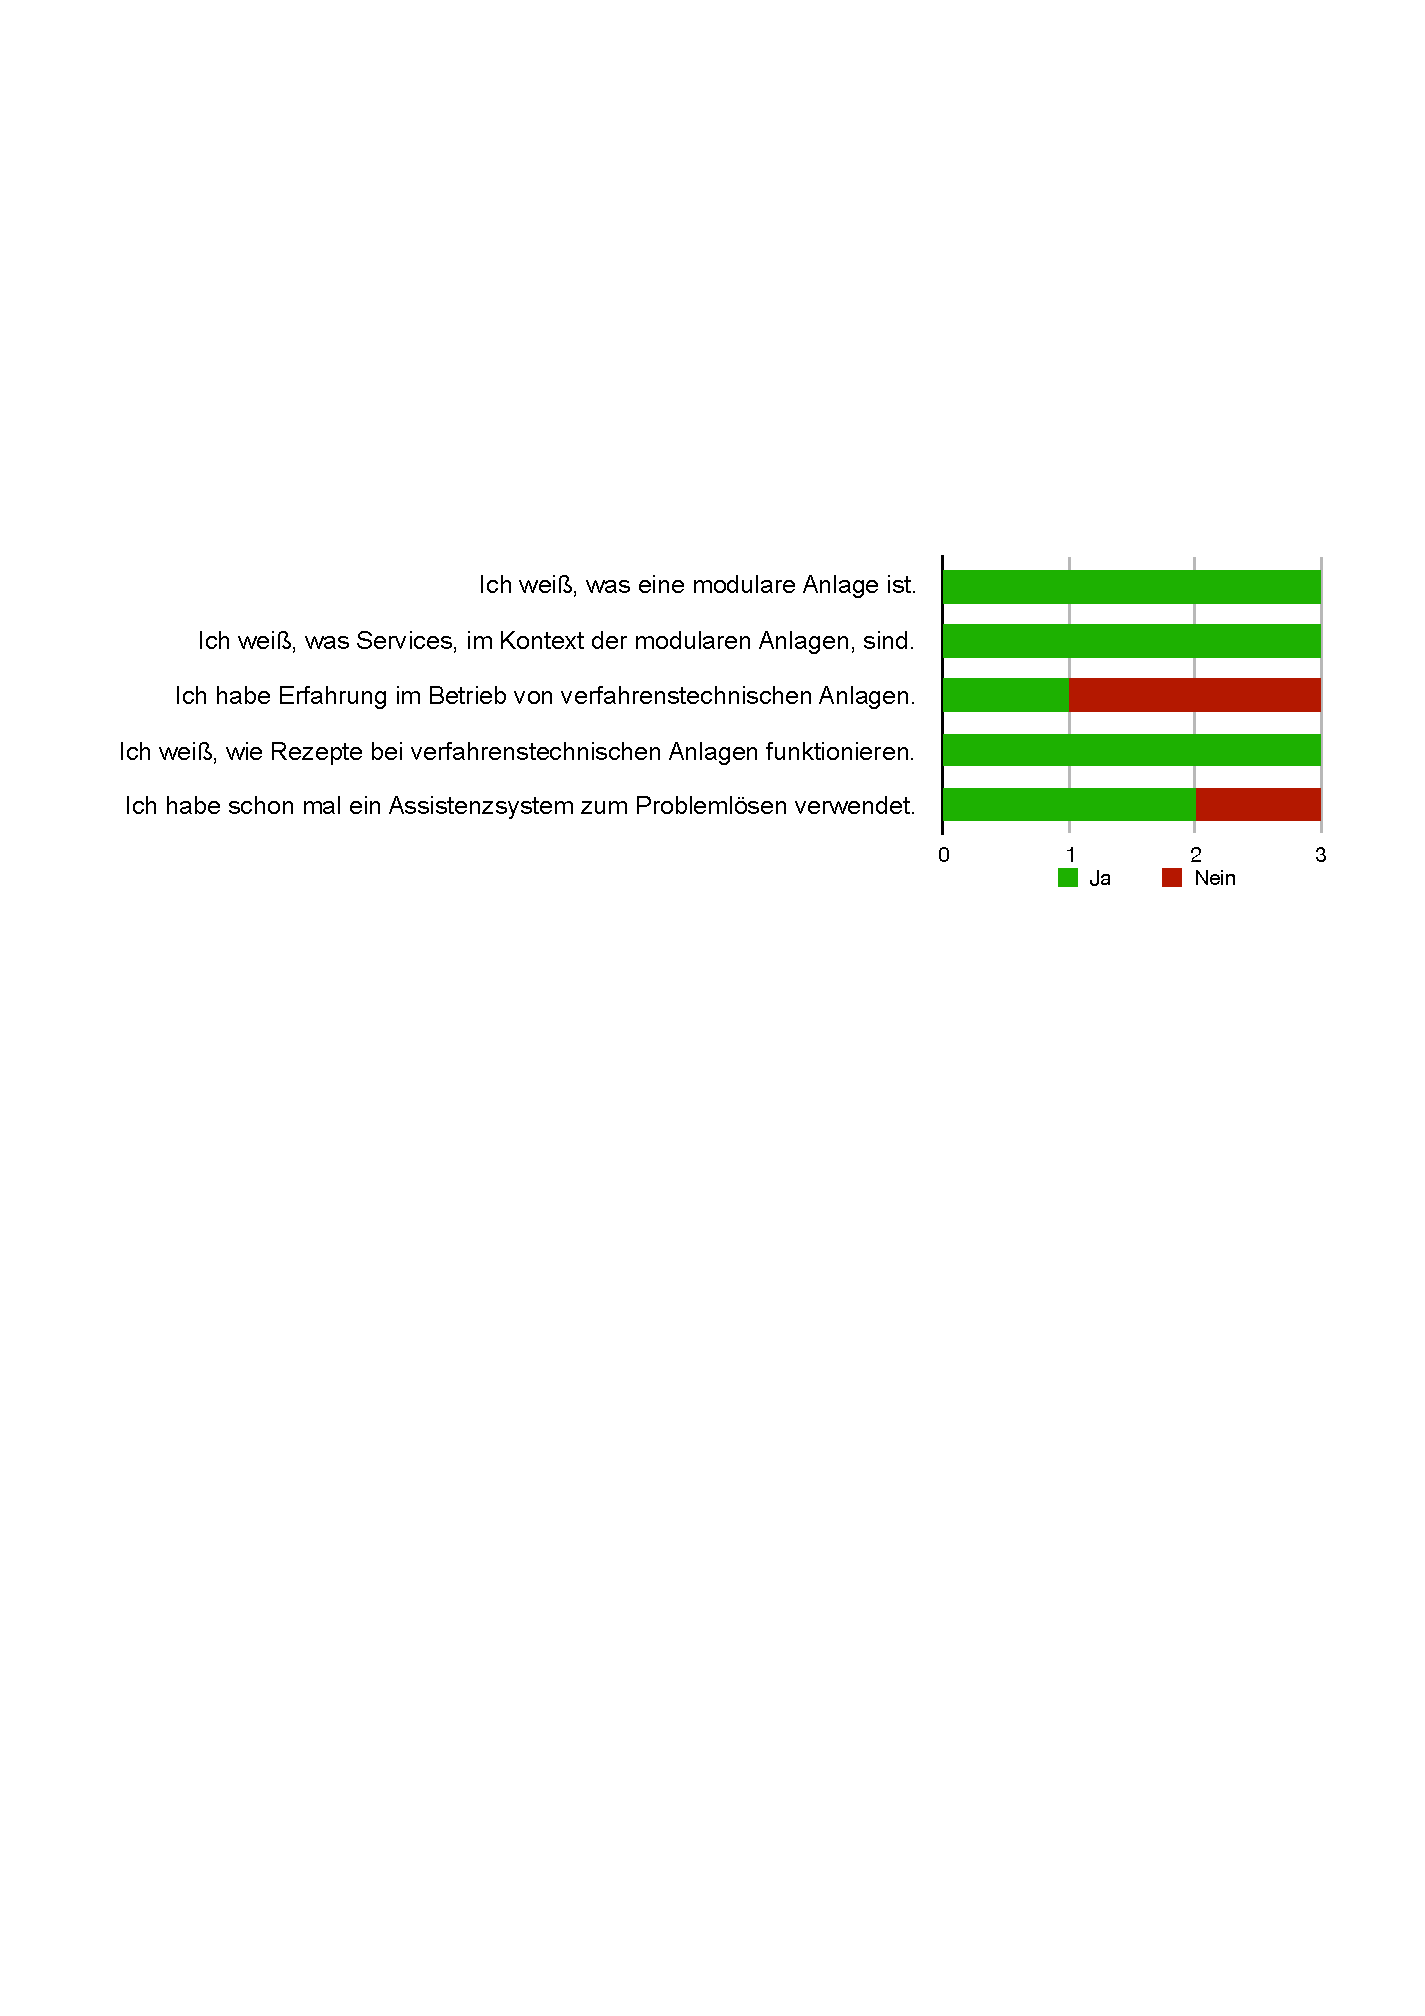
\includegraphics[scale=0.65]{DA_files/Bilder/Validierung/Bild-Vorwissen.pdf}
\caption{Vorwissen zu modularen Anlagen und Assistenzsystemen}
\label{pic:Fragebogen-Vorwissen}
\end{figure}

Die Gesamtauswertung des SUS Fragebogens liefert einen Wert von 75,8. Auf der Skala von 0 bis 100 ist dieser Wert insgesamt als positiv zu bewerten.  Auffällig ist, dass alle Experten bei der Bedienung des Assistenzsystems etwas unsicher waren (siehe Abbildung \ref{pic:SUS-positiv}). Laut deren Aussage lag das vor allem an versteckten Funktionalitäten. Von keinem der Experten wurde die Möglichkeit gefunden ein Ziel zu löschen. Es war nicht ersichtlich, dass man ein Ziel überhaupt löschen kann. Ideen der Experten sind zum einen das Mülleimer-Symbol auszugrauen und hervorzuheben, wenn man ein Ziel markiert. Zum anderen wurde gewünscht ein Ziel direkt mit einem Kreuz am rechten Rand zu löschen \todo{Bild}. Ebenfalls nicht ersichtlich war für einen Experten die Möglichkeit zurück zu navigieren. Warum die Funktion nicht im ersten Schritt gefunden wurde, konnte nicht geklärt werden. Die größte Schwierigkeit bestand in der Entscheidungsfindung. Alle merkten an, dass sie gerne eine Gesamtübersicht der Kosten hätten. Sie erhoffen sich davon besser abschätzen zu können, was die beste Variante ist. Der Prototyp bietet ideale Voraussetzung zu überprüfen, wie sich die Entscheidung bei unterschiedlich bereitgestellten Informationen verändert.
\begin{figure}[htb]
\centering
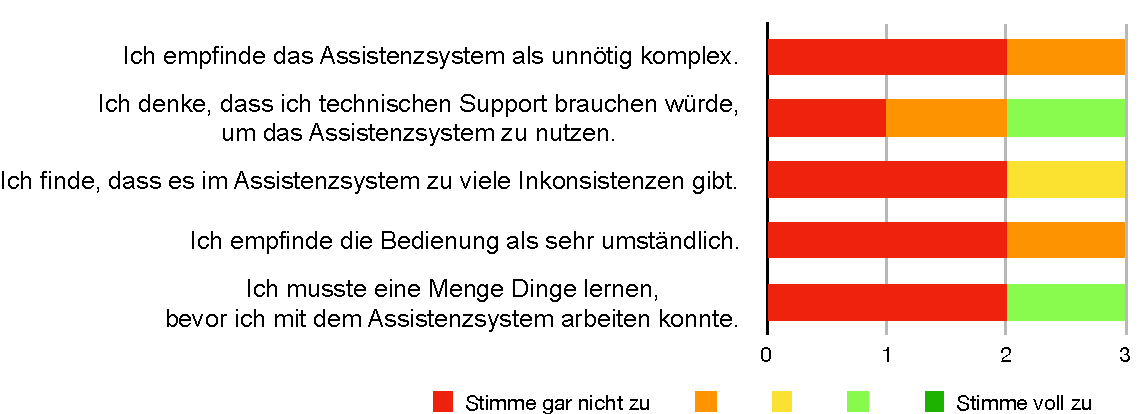
\includegraphics[scale=0.65]{DA_files/Bilder/Validierung/Bild-negative_Aussagen.pdf}
\caption{Bewertung negativer Aussagen SUS Fragebogen}
\label{pic:SUS-negativ}
\end{figure}

Die Experten sind sich einig, dass die meisten Leute das Assistenzsystem schnell beherrschen können (siehe Abbildung \ref{pic:SUS-positiv}). Gelobt wurden dabei der schlichte Aufbau und die grundsätzlich einfache Bedienung. Ebenfalls positiv kam die Vorauswahl an Zielen und Lösungen an \todo{umformulieren}, da diese den Nutzer leiten können. Wenn der Nutzer sich vollständig selber überlegen muss, welche Ziele wichtig und welche Lösungen möglich sind, rechnen die Experten mit Konflikten. Insgesamt schätzen die Experten die Menge an Informationen als sehr gut ein und können sich vorstellen das Assistenzsystem regelmäßig zu nutzen.
\begin{figure}[htb]
\centering
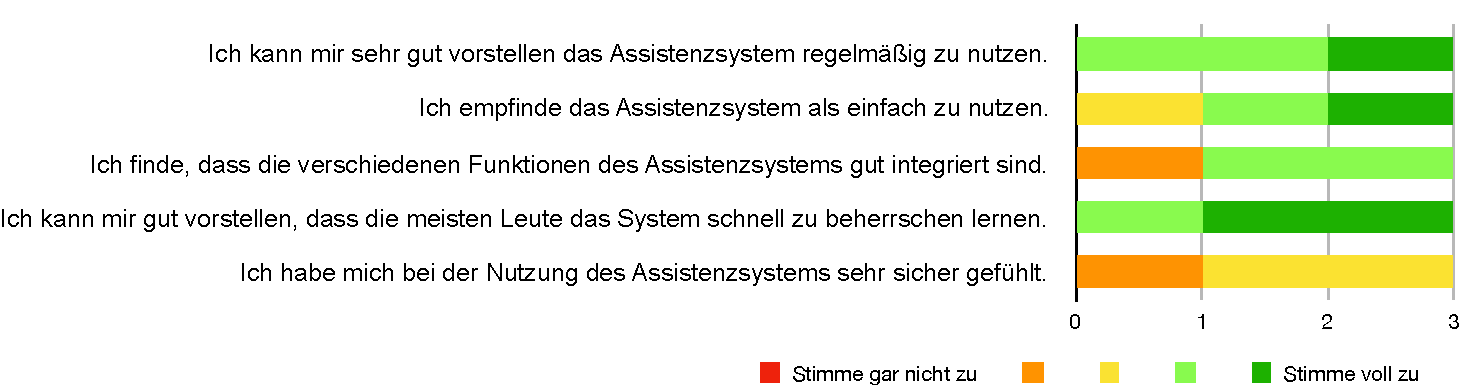
\includegraphics[scale=0.55]{DA_files/Bilder/Validierung/Bild-positive_Aussagen.pdf}
\caption{Bewertung positiver Aussagen SUS Fragebogen}
\label{pic:SUS-positiv}
\end{figure}

\subsubsection*{Weitere gewünschte Funktionalitäten}
Für eine noch umfangreichere Anwendung des Assistenzsystems wünschen sich einige Experten die Integration von weiteren Funktionen. Insbesondere hervorzuheben ist die Unterstützung bei der Anwendung der Lösung. Dadurch kann der Nutzer genau erkennen, welchen Einfluss seine Entscheidung hat und auch bewerten, wie gut diese war. Ein Experte erhofft sich damit, bei ähnlichen Problemen auf Erfahrungswerte zurück greifen zu können. Dieser wünscht auch, dass das Assistenzsystem mitteilt, ob nach einiger Zeit Lösungen weg fallen und wie viele weitere Lösungen es noch gibt. Beispielhaft wurde die erste Lösungsoption im Use Case genannt. Diese ist nur anwendbar, wenn der Nutzer die Entscheidung fünf Tage vor dem Austausch trifft. Entscheidet er sich erst später soll ihm bereits vorher mitgeteilt werden, dass sich die Menge an Lösungen reduziert. \todo{Schlusssatz}

\section{Bewertung}
Die Validierung des Prototypen zeigt ein insgesamt positives Ergebnis. Das Assistenzsystem begleitet den Nutzer durch den Problemlöseprozess, indem es auf Probleme aufmerksam macht und Lösungen aufzeigt. Eine noch größere Bandbreite an Lösungen kann generiert werden, wenn der Nutzer selber Lösungen eingeben kann. Auch könnte die Qualität der angezeigten Lösungen verbessert werden, wenn eindeutig wird, welche Informationen ein Unternehmen beim Betrieb der modularen Anlage zwingend benötigt. Der Prototyp bietet die Grundlage für eine Untersuchung, welche dargestellten Informationen den Nutzer bei der Entscheidungsfindung beeinflussen. Dass dieser dafür geeignet ist, zeigt sowohl die Auswertung der allgemeinen Anforderungen an Assistenzsysteme als auch die Befragung der Experten. Die Grundsätze der Dialoggestaltung wurden eingehalten und auch die Aspekte für die Informationsdarstellung sind erfüllt. Die Umfrage unter den Experten fällt mit einem Schnitt von 75,8, auf einer Skala von 0 bis 100, ebenfalls positiv auf. Besonders gelobt wurde die Übersichtlichkeit und die leichte Bedienbarkeit. Kritik übten die Experten an einzelnen versteckten Funktionen, welche dem Nutzer besser sichtbar gemacht werden sollten. Werden diese noch integriert steht ein Anwendung der entwickelten Nutzeroberfläche nicht mehr viel im Weg \todo{positiver!}.
